\chapter{Thread Domains}
\label{chapter:threaddomains}

ACE is split into three distinct layers. Events are passed from layer to
layer over well-defined interfaces. The responses to these events are often 
passed over
a different interface back to the calling layer. Most of these interfaces
have methods with a void return type. Instead of waiting for a method
to complete its execution, these method calls could be executed 
asynchronously by
another thread. This allows the caller thread to process another event
in the layer.

The prime reason to invoke methods asynchronously arouse in the session server
logic of the collaboration layer. The processing of incoming requests
must be serialized, that is only one request at a time is processed by
the logic (see \ref{chapter:algorithm}). However, the sending of the
resulting transformed requests to the other participants should be executed
on another thread because a slow network connection to one participant
should not slow down the whole processing of requests on the server and thus
the whole editing session.

The problems described above lead us to think about a general solution that 
solves them as well as some other related problems.



\section{Introduction}

\subsection{Requirements}
There were several requirements for designing the thread domain concept.

\begin{itemize}
 \item asynchronous method invocations (invoke and forget)
 \item general applicability
 \item flexible thread creation, reuse of threads
 \item keep code testable in presence of potential multithreading
\end{itemize}

\subsubsection{Asynchronous Method Invocation}
The most important requirement was asynchronous method invocation. 
The caller of methods with a void return type often does not want to wait
for the end of the execution. Thread domains provide a solution to that
problem.


\subsubsection{Generally Applicability}
It would be easy to achieve the asynchronous method invocation requirement
with custom code. One naive solution consists in simply implementing the target
interface by creating and starting a thread which then does the method
invocation.

\small{\begin{verbatim}
 public class ServiceProxy implements Service {
   protected Service target;
   public void doService(final String message) {
     new Thread() {
       public void run() {
         target.doService(message);
       }
     }.start();
   }
 }
\end{verbatim}}

Implementing this pattern whenever an asynchronous invocation is desired
is tedious at best. The obvious problem of starting a new thread
each time a method is invoked could be remedied by the use of an
executor service using a thread pool (Java 1.5).

\small{\begin{verbatim}
 public class ServiceProxy implements Service {
   protected Service target;
   protected ExecutorService executor;
   public void doService(final String message) {
     executor.execute(new Runnable() {
       public void run() {
         target.doService(message);
       }
     });
   }
 }
\end{verbatim}}

However, this solution is still less than ideal, because it needs custom code
to invoke each target method. Further, this has nothing to do with the
target objects logic. In AOP (aspect oriented programming) parlance this
is clearly a cross-cutting concern. Invoking methods asynchronously can 
be applied to any object, no matter how it is implemented. The implementation
of the \texttt{Runnable} above can be created once and for all using the
facilities provided by dynamic proxies and reflection. It is therefore
required that the implemented solution is generally applicable.

\subsubsection{Flexible Thread Creation}
Placing thread creation code in a lot of different places in an application
makes it difficult to manage and tune the usage of threads (see for instance
the code example above). Thread domains should help to control the
number and reuse of threads in a flexible way.

\subsubsection{Testability}
One drawback of introducing multithreading in a codebase is loss of
testability. As soon as there are multiple threads in a system, it is
hard to create deterministic tests, thus resulting in a less testable
system. Therefore, thread domains should help to introduce multithreading
without sacrificing testability.


\subsection{Idea}
The idea of a thread domain is to create a dynamic proxy which stands
in for a real target object. The dynamic proxy is responsible that the
invocation is invoked by another thread, a so called worker thread. 

A thread domain provides a way to wrap an existing object with a dynamic
proxy object, which in turn takes care that the invocations to the
target object are carried out inside the thread domain (i.e. by a 
dedicated worker thread).

With a thread domain that has a single worker thread it is possible to ensure
that only one thread executes code in that subsystem. To achieve that, the
programmer has to wrap all incoming references to that subsystem with
the dynamic proxies created by the thread domain.

If thread domains are simply used to
invoke methods asynchronously such measures have not to be taken. The
concept is still applicable and useful though.


\subsection{Basic Design}
\label{sect:threaddomain.introduction.principle}
Figure \ref{fig:threaddomain_basic} shows the principle of thread domains.
The first object is a dynamic proxy, which is responsible to
capture all the necessary information so that the method invocation can
be executed at a later point. This includes the target object, the method
to be invoked, as well as all the method parameters. This proxy then adds
the method invocation to a queue. After these few steps the proxy returns
to the caller. As there is no return value available from the method 
invocation (the real method has not been invoked yet), the proxy returns
null, zero, or false depending on the return type of the
invoked method.

A worker thread is waiting on the blocking queue for method invocations.
Whenever a method invocation is available that method invocation object
is removed from the queue and executed on the worker thread. 

\begin{figure}[H]
 \centering
 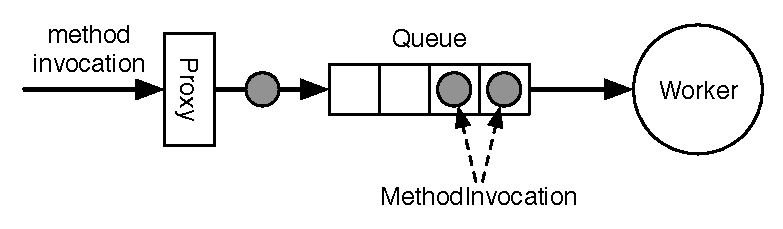
\includegraphics[width=12.7cm,height=3.32cm]{../images/finalreport/threaddomain_basic.eps}
 \caption{Basic Thread Domain Architecture}
 \label{fig:threaddomain_basic}
\end{figure}



\section{Implementation}

\subsection{ThreadDomain Interface}
The core interface is \texttt{ch.\-iserver.\-ace.\-util.\-ThreadDomain} 
(see figure \ref{fig:threaddomain_interface}). Thread domains can be given
a name, which is useful for debugging purposes. The worker threads created
from a thread domain are given a name derived from the name of the thread
domain.

However, the most important methods exposed by that interface are the 
\texttt{wrap} methods. These methods allow wrapping an object so that all 
method invocations on that object are executed inside the thread domain. This 
interface is the only interface users of thread domains need to know. The
second \texttt{wrap} method has a flag parameter that indicates whether
methods with non-void return type should be executed asynchronously (resulting
in an invalid return value) or synchronously.

Thread domains could be extended to make the selection of methods that should
be executed asynchronously even more flexible. This was not required in
the diploma project, thus there is no such facility.

\begin{figure}[H]
 \centering
 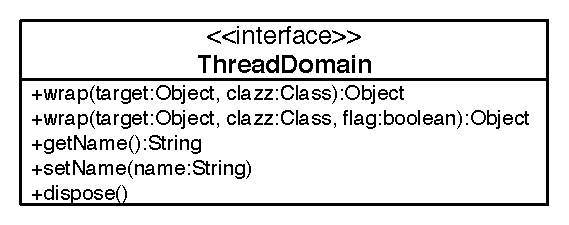
\includegraphics[width=9.07cm,height=3.25cm]{../images/finalreport/threaddomain_uml.eps}
 \caption{ThreadDomain interface}
 \label{fig:threaddomain_interface}
\end{figure}

The \texttt{dispose} method disposes the thread domain, shutting down 
created worker threads and releasing resources used by the thread domain.

The exact implementation of thread domains can vary significantly. The most 
significant differences are found in the management of worker threads.


\subsection{Proxy Implementation}
One of the requirements was that thread domains should work universally across
different classes. This is achieved by the use of the facilities provided by
Java 1.3, namely dynamic proxies. Although the implementation does not use
these dynamic proxies directly, it uses them through the Spring AOP facilities.

The code to \emph{wrap} an object in a thread domain can be found in the
abstract base class \texttt{ch.iserver.ace.util.AbstractThreadDomain}. The
core classes used in the protected \texttt{wrap} methods are the
\texttt{org.springfactory.aop.framework.ProxyFactory} class and the 
\texttt{org.aopalliance.intercept.MethodInterceptor}. 

The proxy implementation is found in 
\texttt{ch.iserver.ace.util.AsyncInterceptor}. This class implements the
\texttt{MethodInterceptor} interface, which is part of the AOP Alliance
standard API for aspect oriented programming. The use of the AOP 
infrastructure allows greater flexibility than the standard Java 1.3 dynamic
proxies. First of all, the interceptors can be applied selectively to
methods of an interface. This is used to optionally execute methods with 
a non-void return type synchronously. Otherwise these methods return
the default value of the corresponding type.


\subsection{Worker Thread}
The worker thread, which waits for incoming method invocations to be
executed, is implemented in \texttt{ch.\-iserver.\-ace.\-util.\-AsyncWorker}.

Exceptions thrown by the method invocations cannot be thrown back at the
original caller. An implementation of the 
\texttt{ch.\-iserver.\-ace.\-util.\-AsyncExceptionHandler} can be 
registered with
workers. These exception handlers are notified whenever an invocation
throws an exception. The interface defines a single method named
\texttt{handleException} with a parameter of type 
\texttt{Async\-Execution\-Exception}. This exception has a property named
\texttt{invocation}, which returns the initial invocation on the dynamic
proxy which has a stack trace at the moment of the invocation. This is
especially useful in debugging to pin down the location of the failure.


\subsection{Thread Domain Implementations}
There are several existing thread domain implementations:
\begin{itemize}
 \item caller thread domain
 \item single thread domain
 \item bounded thread domain
 \item isolated thread domain
\end{itemize}

\subsubsection{Caller Thread Domain}
The caller thread domain achieves the goal of maintaining the testability
of the application in spite of multithreading. Each call to a
\texttt{wrap} method simply returns the target object unmodified, thus
method invocations are executed by the caller thread. It
is implemented in the class 
\texttt{ch.\-iserver.\-ace.\-util.\-CallerThreadDomain}.
This class is probably most useful for automatic tests as it does not cause
methods to be invoked on another thread. So, without changing any code
the test can inject this kind of thread domain and test the code
in a fully deterministic way.

\subsubsection{Single Thread Domain}
The single thread domain maintains one worker thread with its associated
queue (see figure \ref{fig:threaddomain.single}). It is implemented in the class
\texttt{ch.\-iserver.\-ace.\-util.\-SingleThreadDomain}.

\begin{figure}[htb]
 \centering
 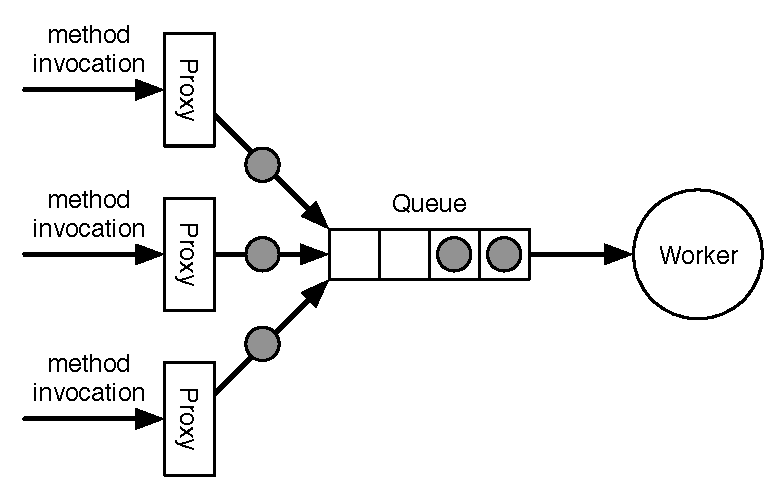
\includegraphics[width=9cm,height=5.55cm]{../images/finalreport/threaddomain_single.eps}
 \caption{Single thread domain - only one shared queue}
 \label{fig:threaddomain.single}
\end{figure}

\subsubsection{Bounded Thread Domain}
The bounded thread domain starts a bounded number of worker threads
(see figure \ref{fig:threaddomain.bounded}). It
is implemented in the class \texttt{ch.iserver.ace.util.BoundedThreadDomain}.
The queues with the associated workers are assigned according to
a round-robin scheme to the proxy objects. The number of worker threads
is bounded and does not grow.

\begin{figure}[htb]
 \centering
 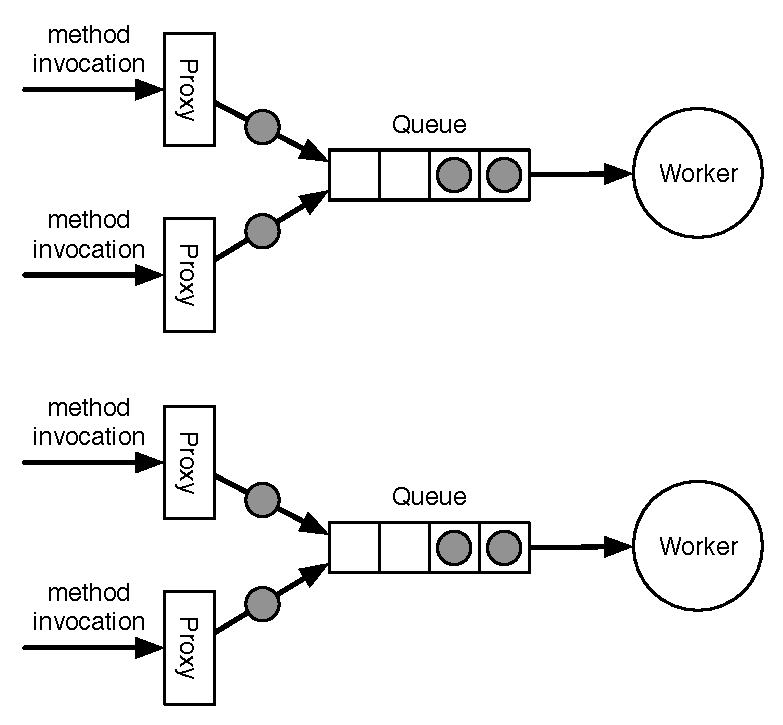
\includegraphics[width=9cm,height=8.3cm]{../images/finalreport/threaddomain_bounded.eps}
 \caption{Bounded thread domain - bounded number of shared queues}
 \label{fig:threaddomain.bounded}
\end{figure}

\subsubsection{Isolated Thread Domain}
The isolated thread domain creates a new queue and associated worker
for each call to the \texttt{wrap} method 
(see figure \ref{fig:threaddomain.isolated}). It is implemented by
\texttt{ch.iserver.ace.util.IsolatedThreadDomain}. This thread domain
uses a weak reference and a reference queue in order to detect when
a worker is no longer needed. A worker thread is no longer needed if the
proxy associated with that worker is only weakly referenced (by a weak
reference from the thread domain). The worker thread can then be
safely stopped. Checking for unused worker threads should happen 
periodically by a collector thread (similar to the garbage collector). The
implementation of this kind of thread domains is in an experimental state.

\begin{figure}[htb]
 \centering
 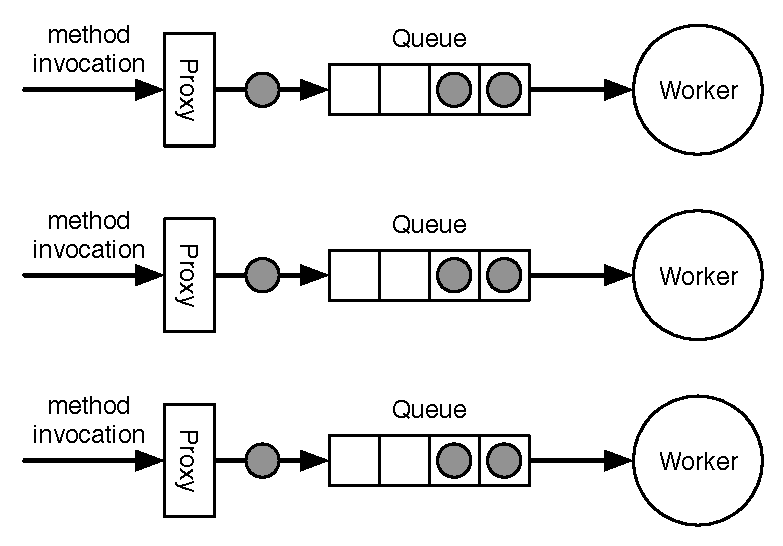
\includegraphics[width=9cm,height=6.15cm]{../images/finalreport/threaddomain_isolated.eps}
 \caption{Isolated thread domain - one queue per wrapped target object}
 \label{fig:threaddomain.isolated}
\end{figure}



\section{Conclusion}

Thread domains proved to be a very useful tool in developing ACE. The
chapter about the collaboration layer describes where and why thread
domains were used (see chapter \ref{chapter:collaborationlayer}).


\subsection{Advantages}
Thread domains have the following advantages:

\begin{itemize}
 \item advantages of threading without loss of testability
 \item applicable to any interface
 \item control over thread creation and usage
 \item asynchronous method invocation
\end{itemize}

One of the biggest advantages is that by replacing the thread domain used
by the code with
a \texttt{CallerThreadDomain} it is possible to test code without any
multithreading. This makes it possible to write unit tests or even 
integration tests that run deterministically.

Thread domains can be used widely with any interface. It is not necessary to
write custom code to asynchronously invoke methods for a new interface type.

Thread domains allow to control how many threads are running in a system.
Thread domain implementations can create worker threads in a flexible way. For
instance a thread pool could be used to create workers. The number of
threads in the pool could shrink or grow, as is needed by the application.

When calling methods with a void return type,
in some cases the caller does not want to wait for the end of the method.
In ACE, sending events over the network may take some time. The collaboration
layer does not want to wait (and block the processing of further events)
until the message is sent. Therefore the use of thread domains makes a
lot of sense.


\subsection{Disadvantages}
Every techniques has its disadvantages:

\begin{itemize}
 \item exceptions are not thrown back at the caller
 \item methods with non-void return type
\end{itemize}

Exceptions are not thrown on the call to the wrapped object (i.e. the
dynamic proxy). All the 
interceptor does is add the method invocation object to a queue. This makes
finding the cause of errors more difficult, as exceptions thrown by the
method invocation do not contain the original caller in the stack trace.
The stack trace at the moment of the invocation of the wrapped object must
be recorded and passed along to the worker thread in order that the worker
thread can report the caller's stack trace. 

Further, exception handling can get more difficult. The caller does not
know whether the call succeeded or not. Usually, this problem can be solved
by adding a failure handler. For an example of this usage see the
description of \texttt{ParticipantConnectionWrapper} and 
\texttt{SessionConnectionWrapper}. Of course, in some situation this
design is not applicable and the usage of thread domains is discouraged.

Methods with a non-void return type are another potential problem. As the
interceptor adds the method invocation to a queue and returns immediately,
it is not possible to return the return value of the method invocation.
Asynchronous method invocations return always null (or the corresponding
default value) for methods with a non-void return type. This can cause
unexpected behavior in the caller's code. Therefore, it is best either to
invoke methods with non-void return type synchronously (see \texttt{wrap}
method with three parameters) or avoid wrapping interfaces that contain
methods with non-void return types unless you are absolutely sure that
what you are doing is safe (i.e. you do not want to use the return value).


\subsection{Possible Improvements}
The pattern employed by the wrapper objects for \texttt{Participant\-Connection}
and \texttt{Session\-Connection} could be generalized 
(see chapter \ref{chapter:collaborationlayer}). That is instead of
writing custom code each time exceptions from the asynchronous method invocation
should be handled in a special way, the exception handling of thread domains
could be improved so that it would be usable in these situations.

In some cases if a target object fails, further calls on that object are not
expected to succeed. However, it is still possible that there are method
invocation objects in the queue. Executing these does not make any sense
in that case, but removing them from the queue is also not very elegant.
A possible solution consists in replacing the 
target object with a null object, that
is an object implementing the same interface but simply ignoring the calls.
The Spring framework's AOP support has the interesting concept of
hot swappable target sources that would fit this situation. Target sources
are asked for the target object each time a method is invoked on the
proxy. The hot swappable target source allows to swap the target with a
null object. For more information about the AOP support of Spring see
the documentation at 
\href{http://www.springframework.org/}{http://www.springframework.org/}.

Additionally to the asynchronous execution model, we could also implement
a synchronous execution model. This would have the advantage that the methods
are still executed by the designated worker thread(s) of the thread domain.
This kind of interception could then even return a value and/or throw
exceptions. Thus synchronous interception would be mainly useful for cases where
we want to ensure that a certain subsystem is only executed by designated worker
threads.
